\chapter{Конструкторский раздел}
В этом разделе будут приведены требования к ПО, схемы реализации алгоритмов,
а также выбранные классы эквивалентности для тестирования ПО.

\section{Требования к ПО}
Ниже будет представлен список требований к разрабатываемому программному обеспечению. 

Требования к входным данным: 
\begin{itemize}
	\item на вход подаётся квадратная матрица расстояний, состоящая из целых чисел;
	\item в матрице как минимум две строки;
	\item матрица может быть не симметричной.
\end{itemize}

Требования к выводу: 
\begin{itemize}
	\item программа должна вывести минимальный путь и соответствующее ему минимальное расстояние.
\end{itemize}

\section{Схемы алгоритмов}
На рисунке 2.1 будет приведена схема реализации алгоритма полного перебора.

На рисунках 2.2-2.3 будет приведена схема реализации муравьиного алгоритма.

\FloatBarrier
\begin{figure}[hp]
	\begin{center}
		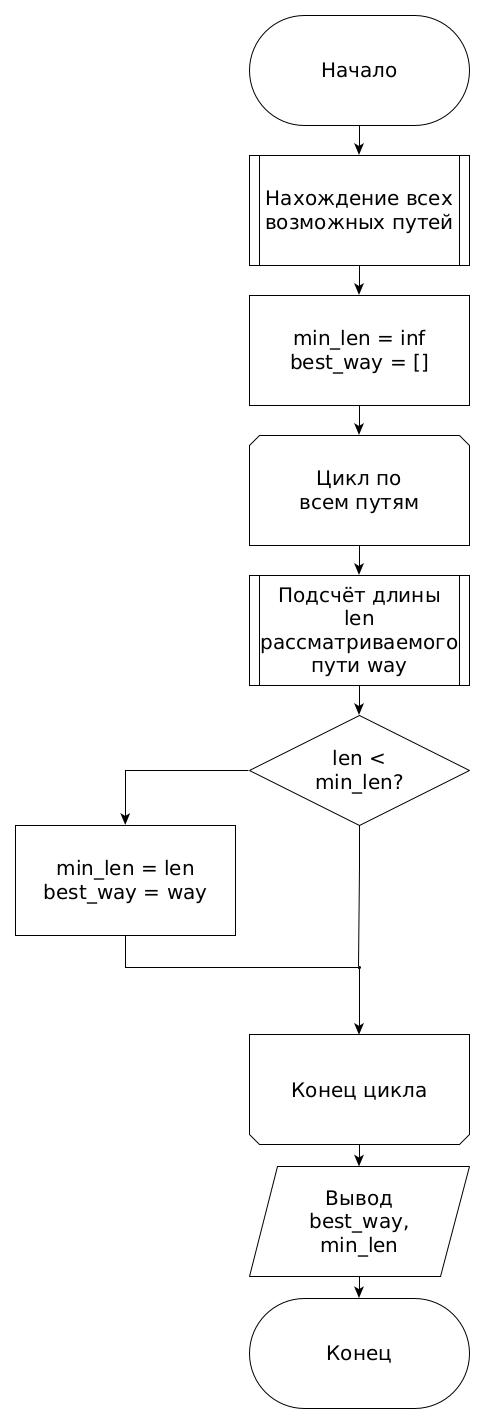
\includegraphics[width=8cm, height=25cm]{graph/full.jpg}
	\end{center}
	\caption{Схема реализации алгоритма полного перебора}
\end{figure}
\FloatBarrier

\FloatBarrier
\begin{figure}[hp]
	\begin{center}
		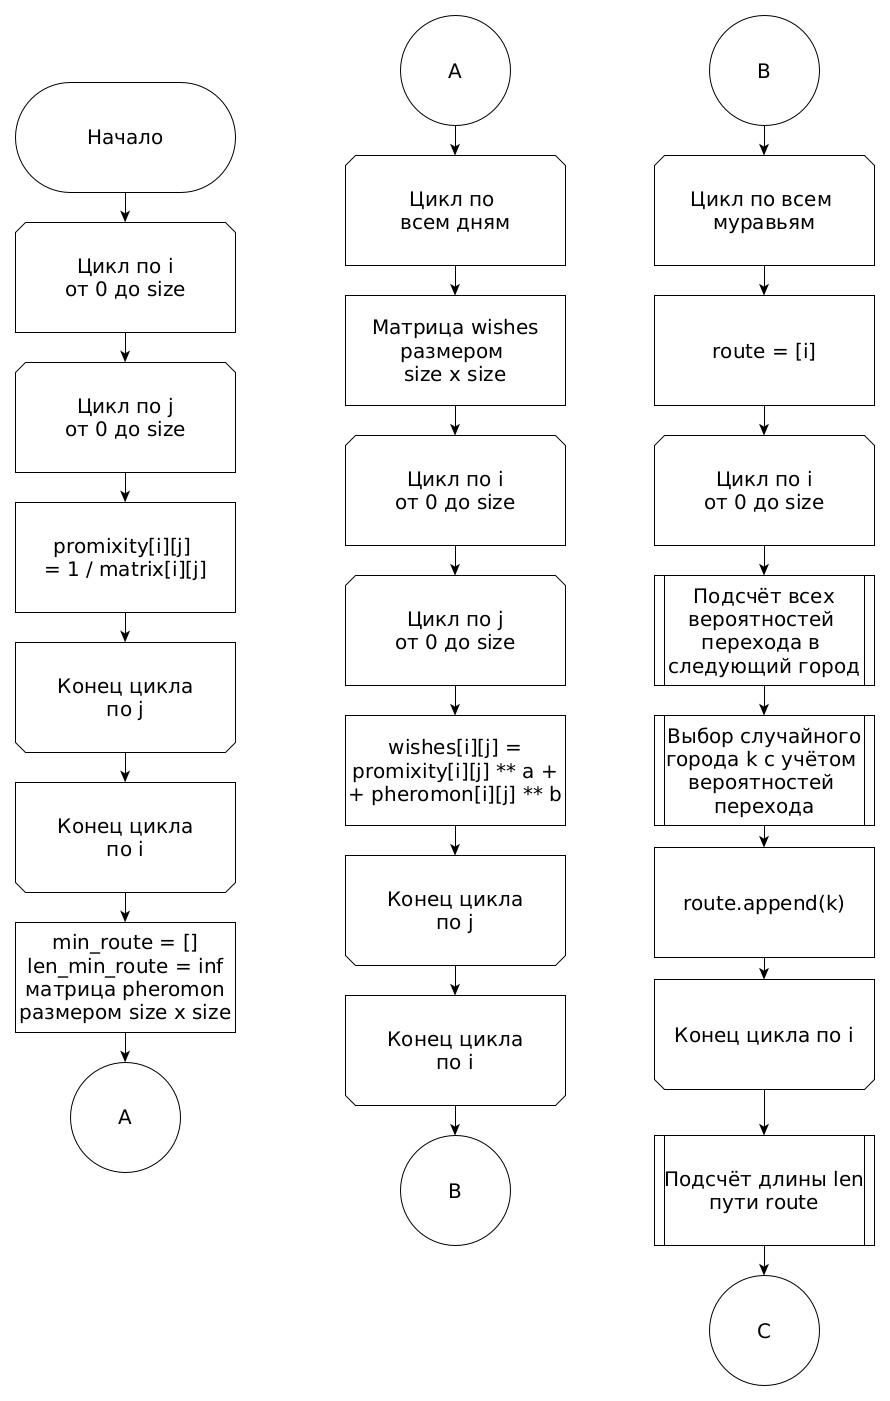
\includegraphics[width=\linewidth]{graph/ant.jpg}
	\end{center}
	\caption{Схема реализации муравьиного алгоритма (часть 1)}
\end{figure}
\FloatBarrier

\FloatBarrier
\begin{figure}[hp]
	\begin{center}
		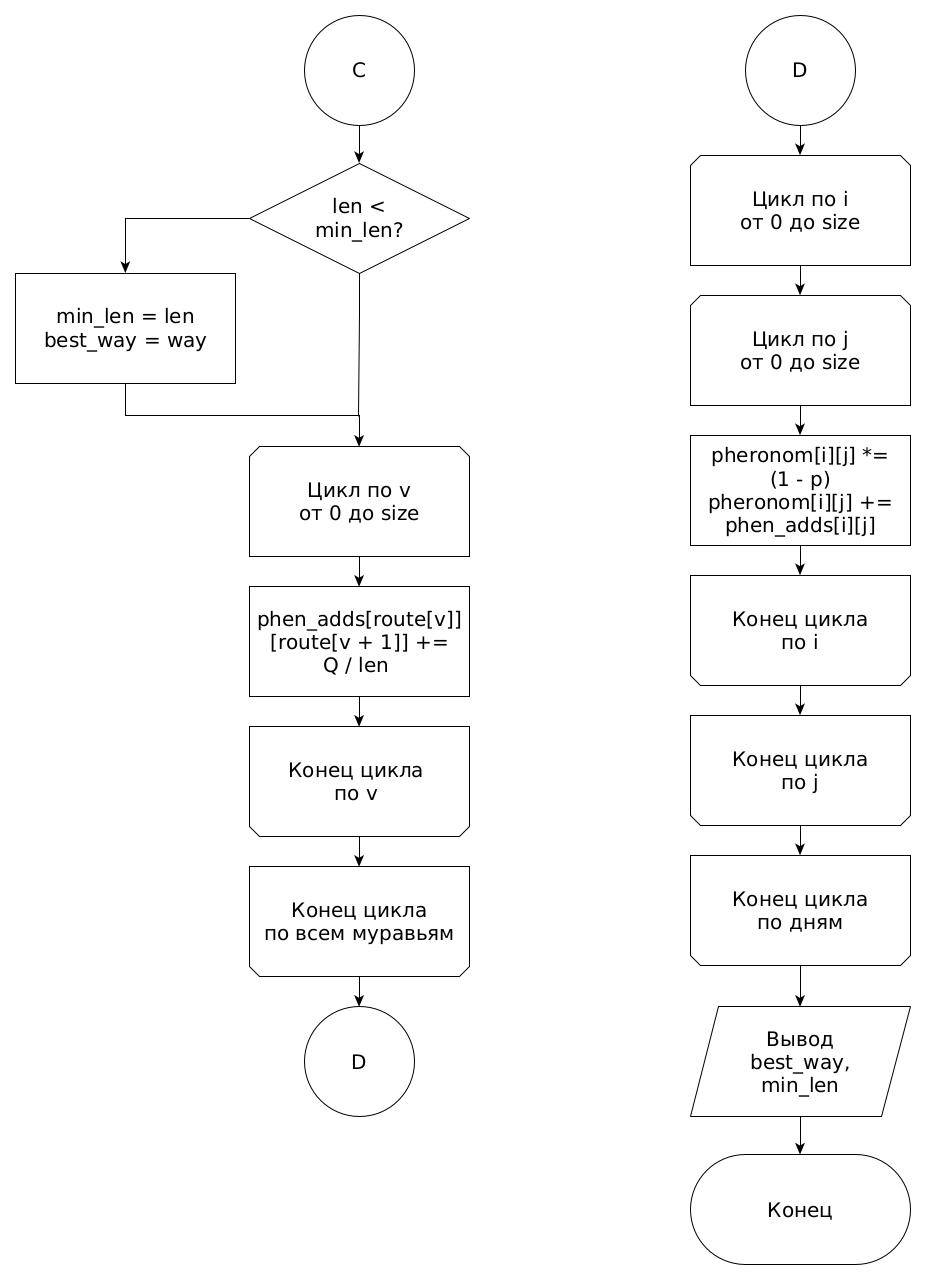
\includegraphics[width=\linewidth]{graph/ant2.jpg}
	\end{center}
	\caption{Схема реализации муравьиного алгоритма (часть 2)}
\end{figure}
\FloatBarrier

\section{Типы данных для алгоритмов}
Тестирование алгоритма будет производиться на матрице из целых чисел.
Тем не менее, алгоритмы универсальны, и для их использования
подходят любые вещественные типы.

Размер массива может быть произвольным из тех, что допустимы по требованиям ко вводу.

\section{Способ тестирования}
Тестирование программы будет произодиться методом чёрного ящика.
Такой подход выбран, так как от реализаций алгоритмов требуется в первую
очередь правильность работы.
Сама по себе реализация не требует тестировки, так как в точности
повторяет теоретические принципы, сформированные в аналитическом
разделе.

В качестве классов эквивалентности были выбраны следующие сущности:
\begin{itemize}
	\item матрица размером 2x2;
	\item матрица размером 5х5;
	\item несимметричная матрица размером 5х5;
	\item матрица, состоящая из одинаковых чисел.
\end{itemize}

\section{Вывод}
Были приведены требования к ПО, схемы реализации алгоритмов.
Был определен способ тестирования алгоритмов.